\section{Auswertung}
\label{sec:Auswertung}
$\theta \rightarrow E$: $E = \frac{hc}{2dn\sin(\theta)}$

\subsection{Bragg-Bedingung}
\label{sec:bragg}

Der Erwartungswert für das Intensitätsmaximum liegt bei $\gamma = 2*theta = 28\si{\degree} $, in diesem Versuch wurde es jedoch bei $26\si{\degree}$ gemessen, wie sich Abb. \ref{fig:bragg} entnehmen lässt.

\begin{figure}
  \centering
  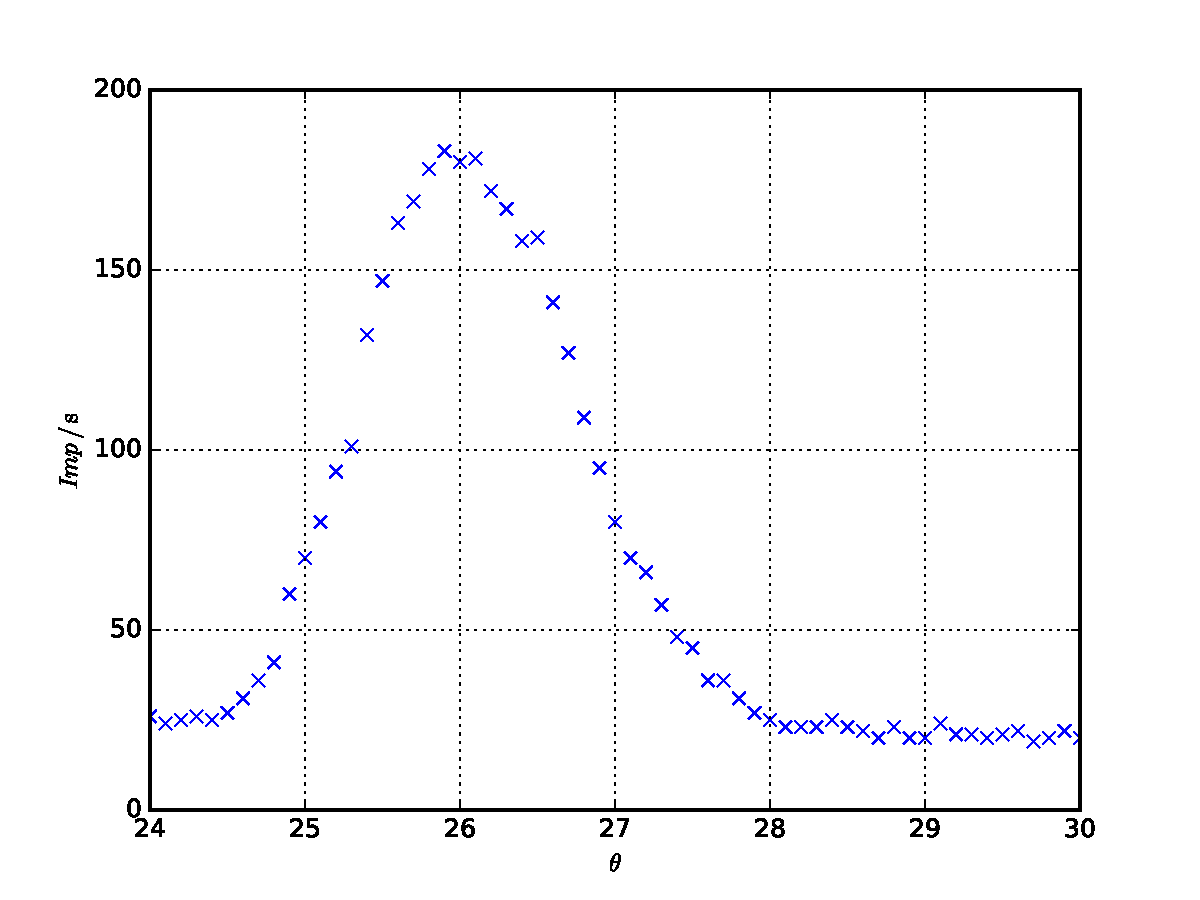
\includegraphics{./Python/bragg.pdf}
  \caption{Zählrate aufgetragen gegen den Winkel $\gamma$ (in Grad) zwischen Röntgenstrahl und Zählrohr bei einem Kristallwinkel von $\theta = 14 \si{\degree}$.}
  \label{fig:bragg}
\end{figure}

\subsection{Emissionsspektrum}
\label{sec:emission}

\begin{figure}
  \centering
  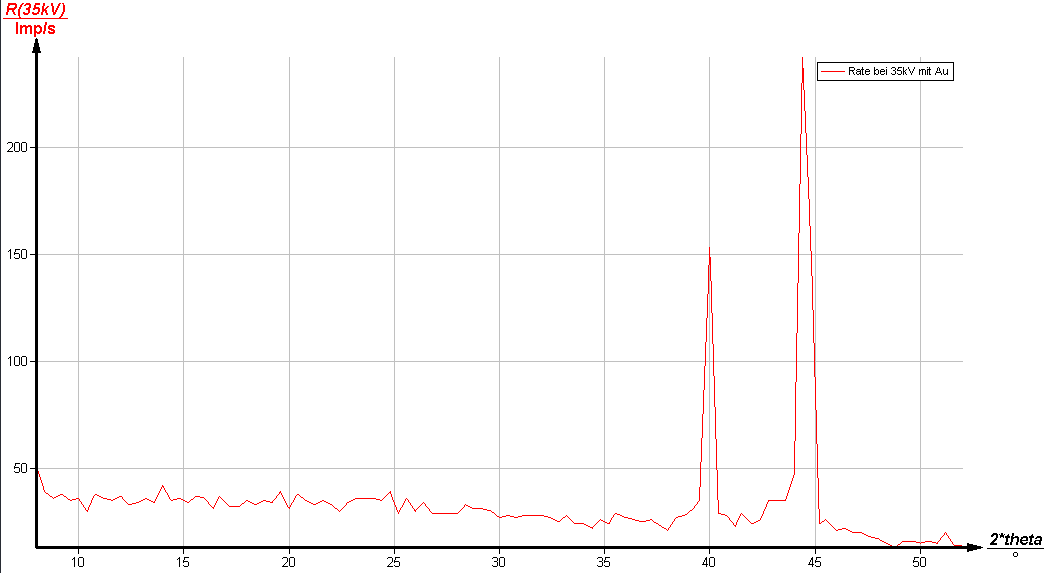
\includegraphics{./Messdaten/Cu.PNG}
  \caption{Gemessenes Röntgenspektrum der verwendeten Kupferröhre}
  \label{fig:brems}
\end{figure}

Die maximale Energie der in der Apparatur auftretenden Röntgenquanten beträgt durch die verwendete Beschleunigungsspannung bedingt $35\symup{keV}$. Es sollte somit im in Abb. \ref{fig:brems} dargestellten Spektrum ein Bremsberg erkennbar sein, dieser lässt sich jedoch nicht nachweisen.

\begin{figure}
  \centering
  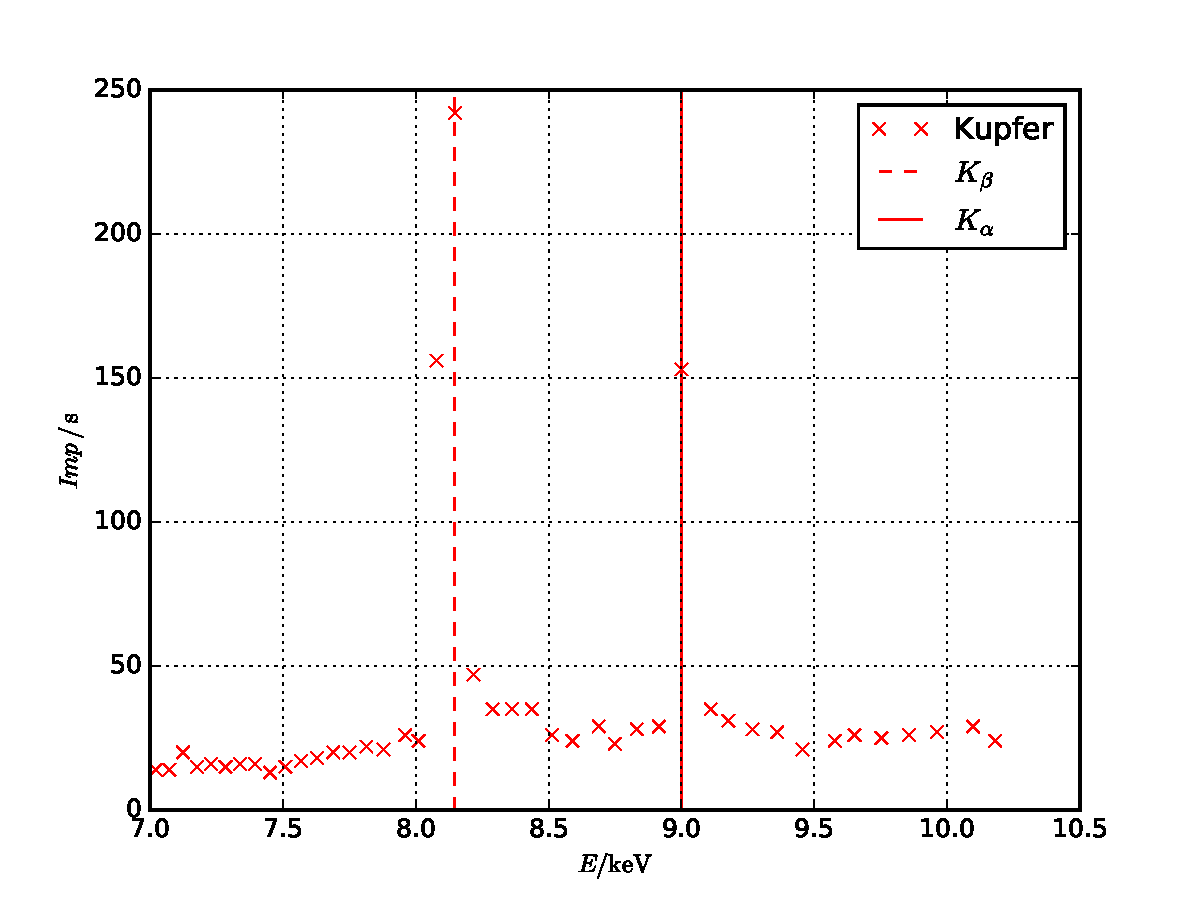
\includegraphics{./Python/Kupfer.pdf}
  \caption{Spektrum der verwendeten Kupfer-Röntgenröhre, eingeschränkt auf $7-10.5 \si{\kilo \electronvolt}$
  \label{fig:klinie}
\end{figure}

Aus Abb. \ref{fig:klinie} lassen sich die Werte $K_\alpha = \SI{9}{\kilo \electronvolt}$ und $K_\beta = \SI{8.15}{\kilo \electronvolt}$ der klar erkennbaren $K_\alpha$- bzw. $K_\beta$-Linie entnehmen.


\subsection{Absorbtionsspektrum}
\label{sec:absorption}

\begin{figure}
  \centering
  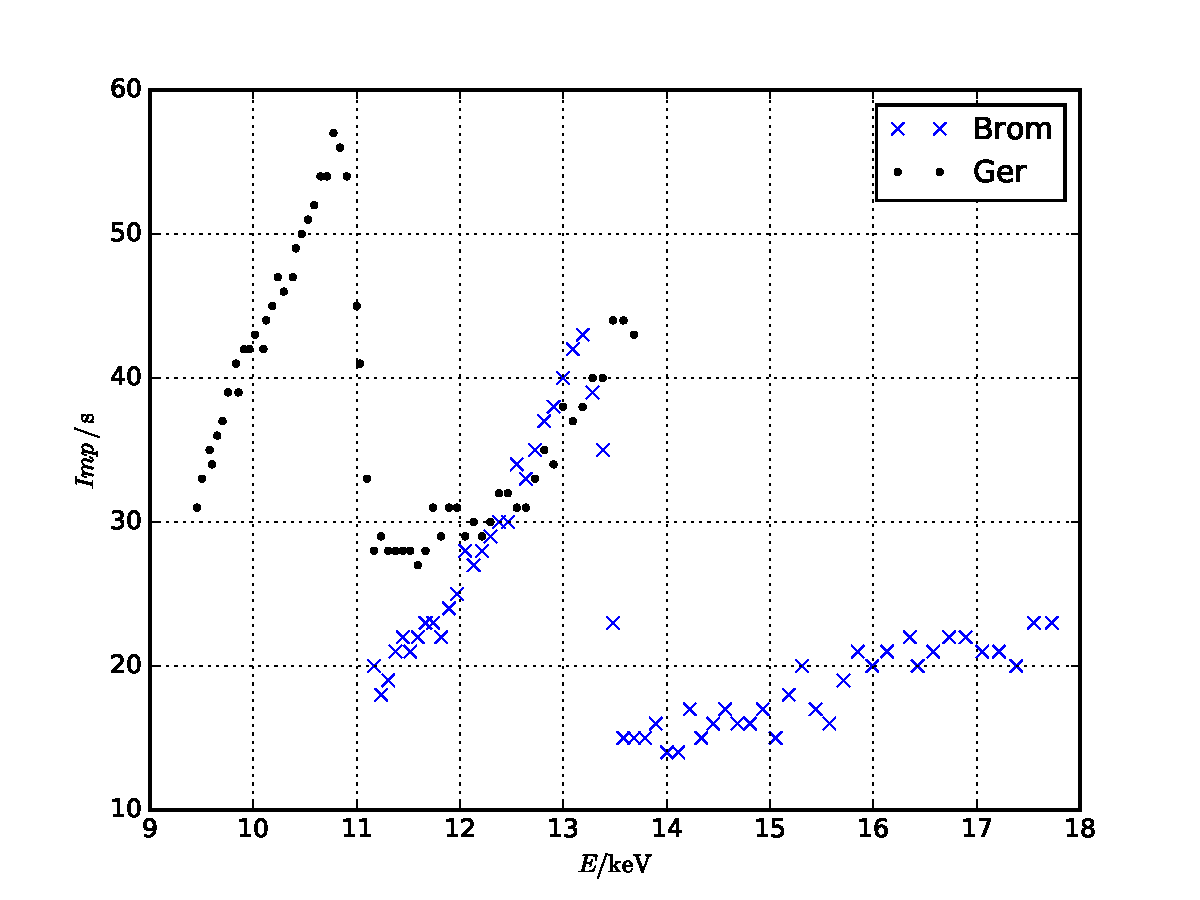
\includegraphics{./Python/Brom.pdf}
  \caption{Messung der vom Kristall gebeugten Röntgenstrahlung unter Verwendung eines Brom-Absorbers.}
  \label{fig:brom}
\end{figure}

\begin{figure}
  \centering
  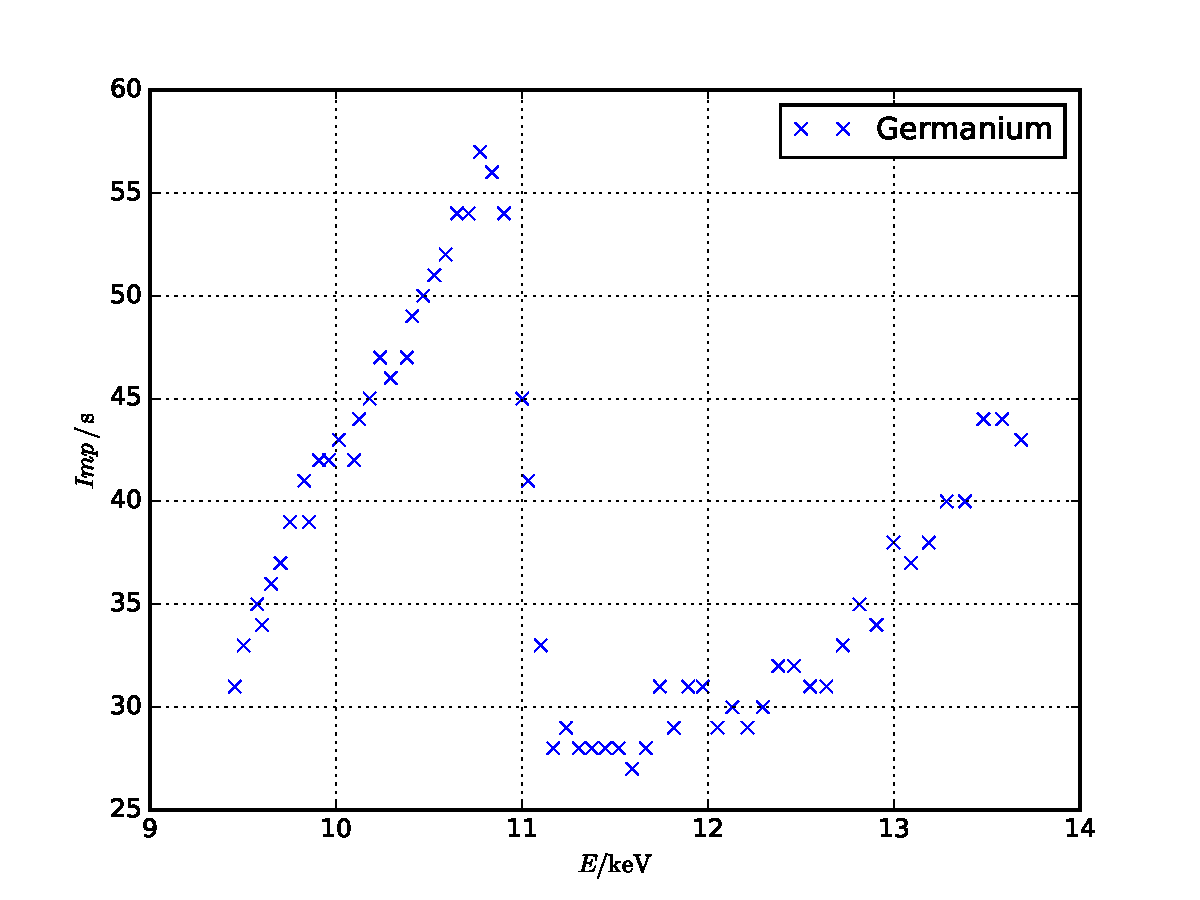
\includegraphics{./Python/Ger.pdf}
  \caption{Messung der vom Kristall gebeugten Röntgenstrahlung unter Verwendung eines Germanium-Absorbers.}
  \label{fig:ger}
\end{figure}

\begin{figure}
  \centering
  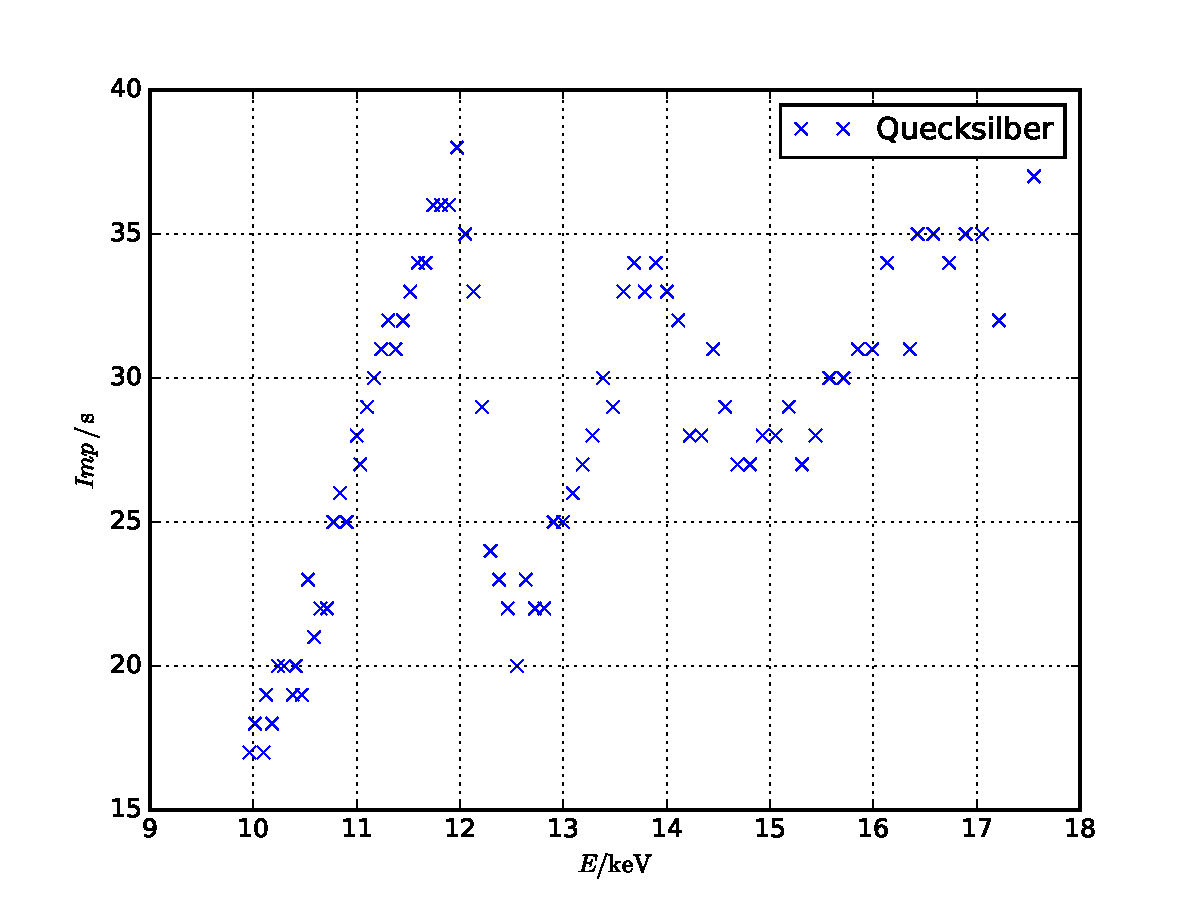
\includegraphics{./Python/queck.pdf}
  \caption{Messung der vom Kristall gebeugten Röntgenstrahlung unter Verwendung eines Quecksilber-Absorbers.}
  \label{fig:queck}
\end{figure}

\begin{figure}
  \centering
  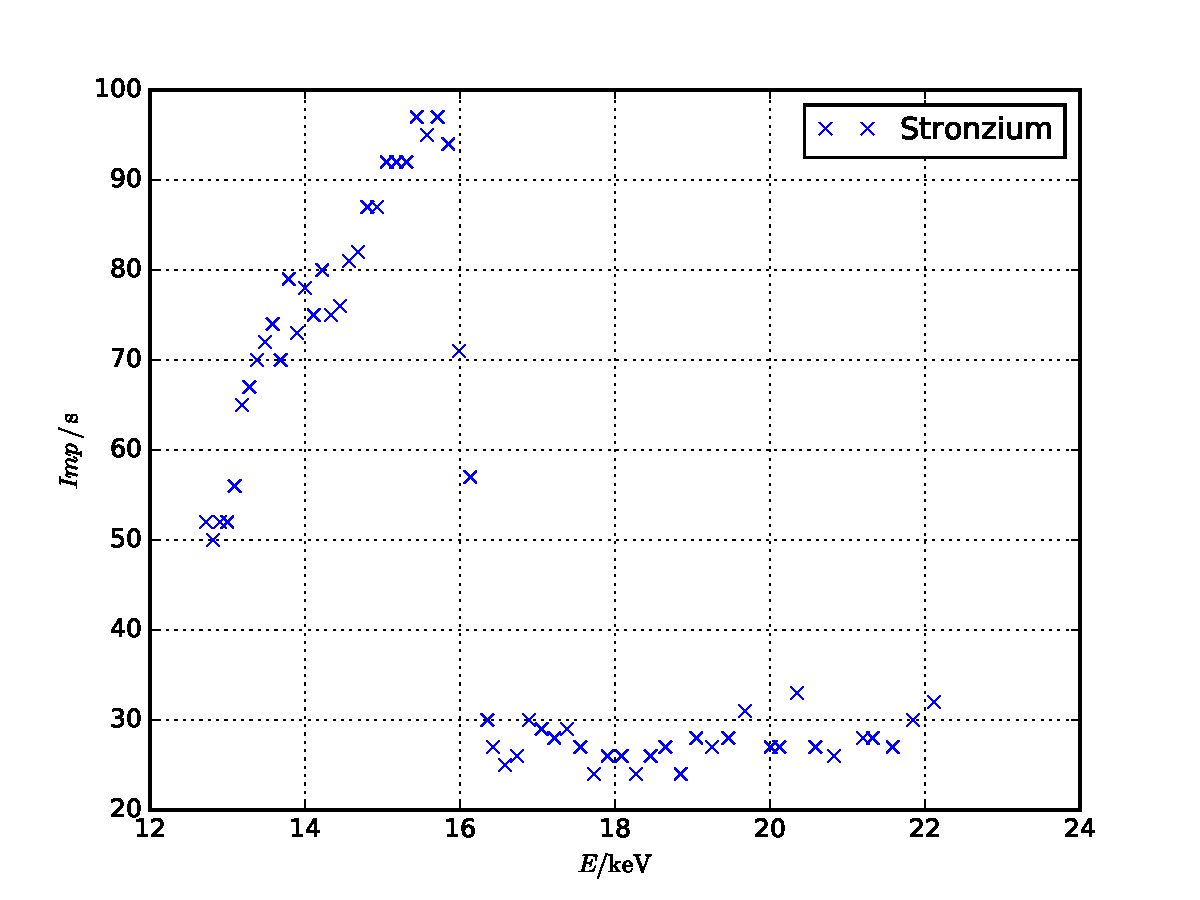
\includegraphics{./Python/stronz.pdf}
  \caption{Messung der vom Kristall gebeugten Röntgenstrahlung unter Verwendung eines Stronzium-Absorbers.}
  \label{fig:stronz}
\end{figure}

\begin{figure}
  \centering
  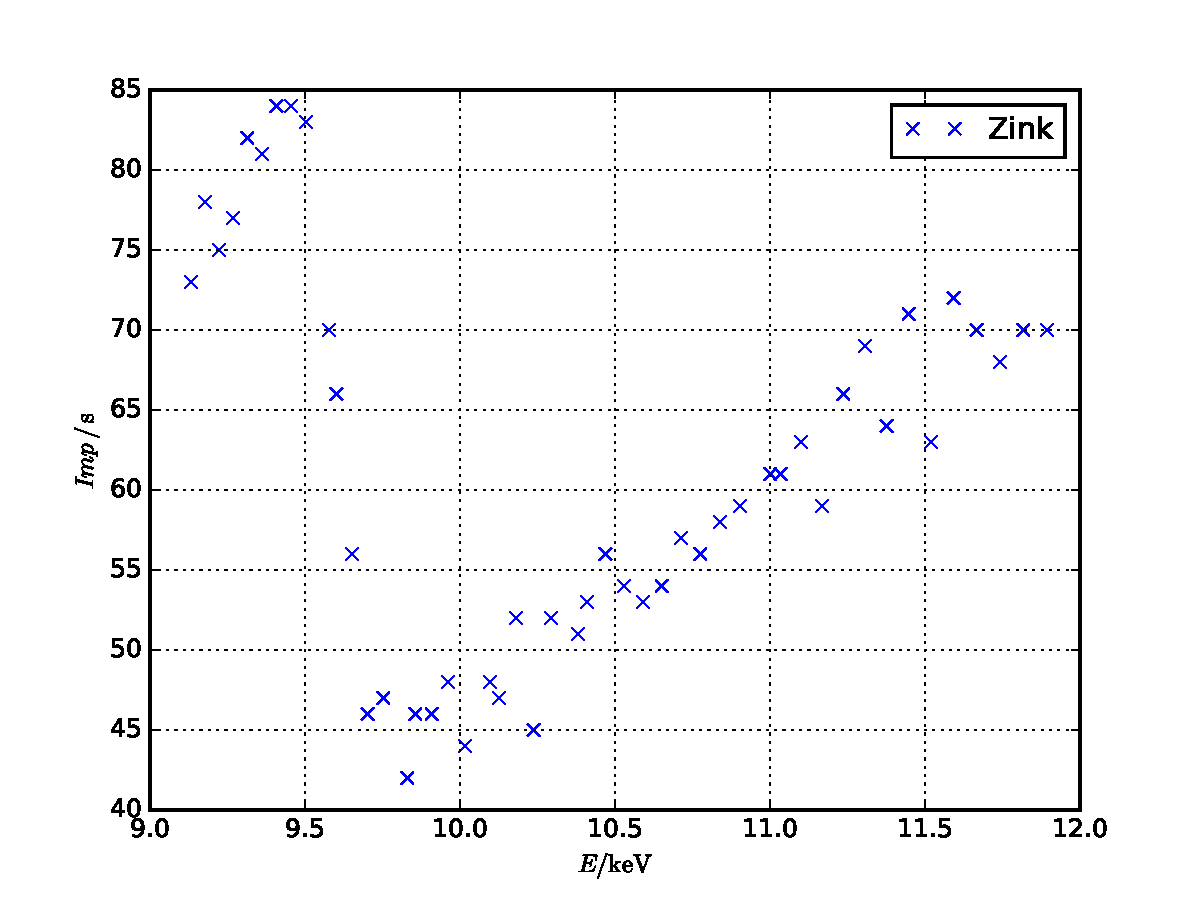
\includegraphics{./Python/zink.pdf}
  \caption{Messung der vom Kristall gebeugten Röntgenstrahlung unter Verwendung eines Zink-Absorbers.}
  \label{fig:zink}
\end{figure}

\begin{figure}
  \centering
  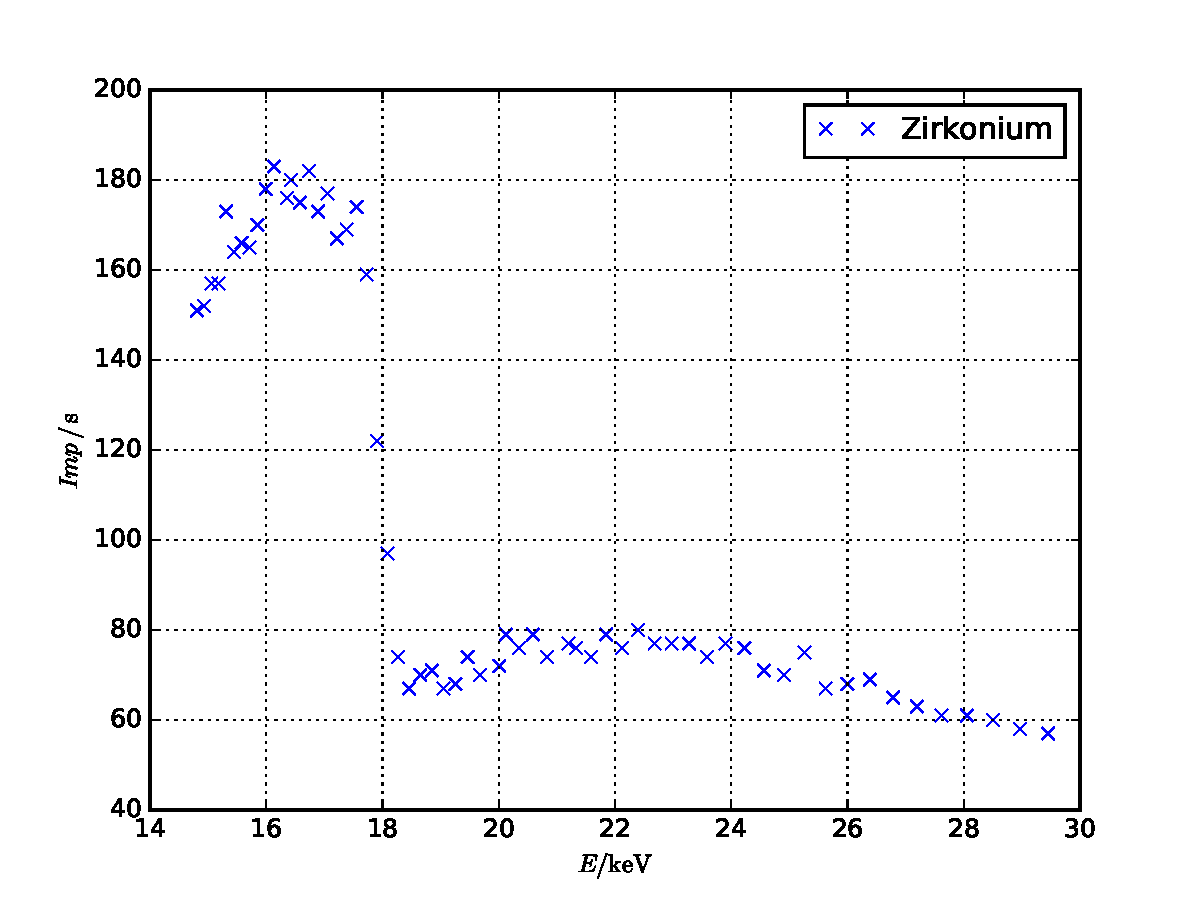
\includegraphics{./Python/zirk.pdf}
  \caption{Messung der vom Kristall gebeugten Röntgenstrahlung unter Verwendung eines Zirkonium-Absorbers.}
  \label{fig:brom}
\end{figure}
